\section{Time Complexity Analysis of Randomized Quicksort}
% ./programs/analysis_quicksort/sorting_algorithms_benchmark.tex
% create a full frame image for this ignore the frame padding pages
\begin{frame}{Sorting Algorithms Benchmark}
  \begin{figure}[h]
    \centering
    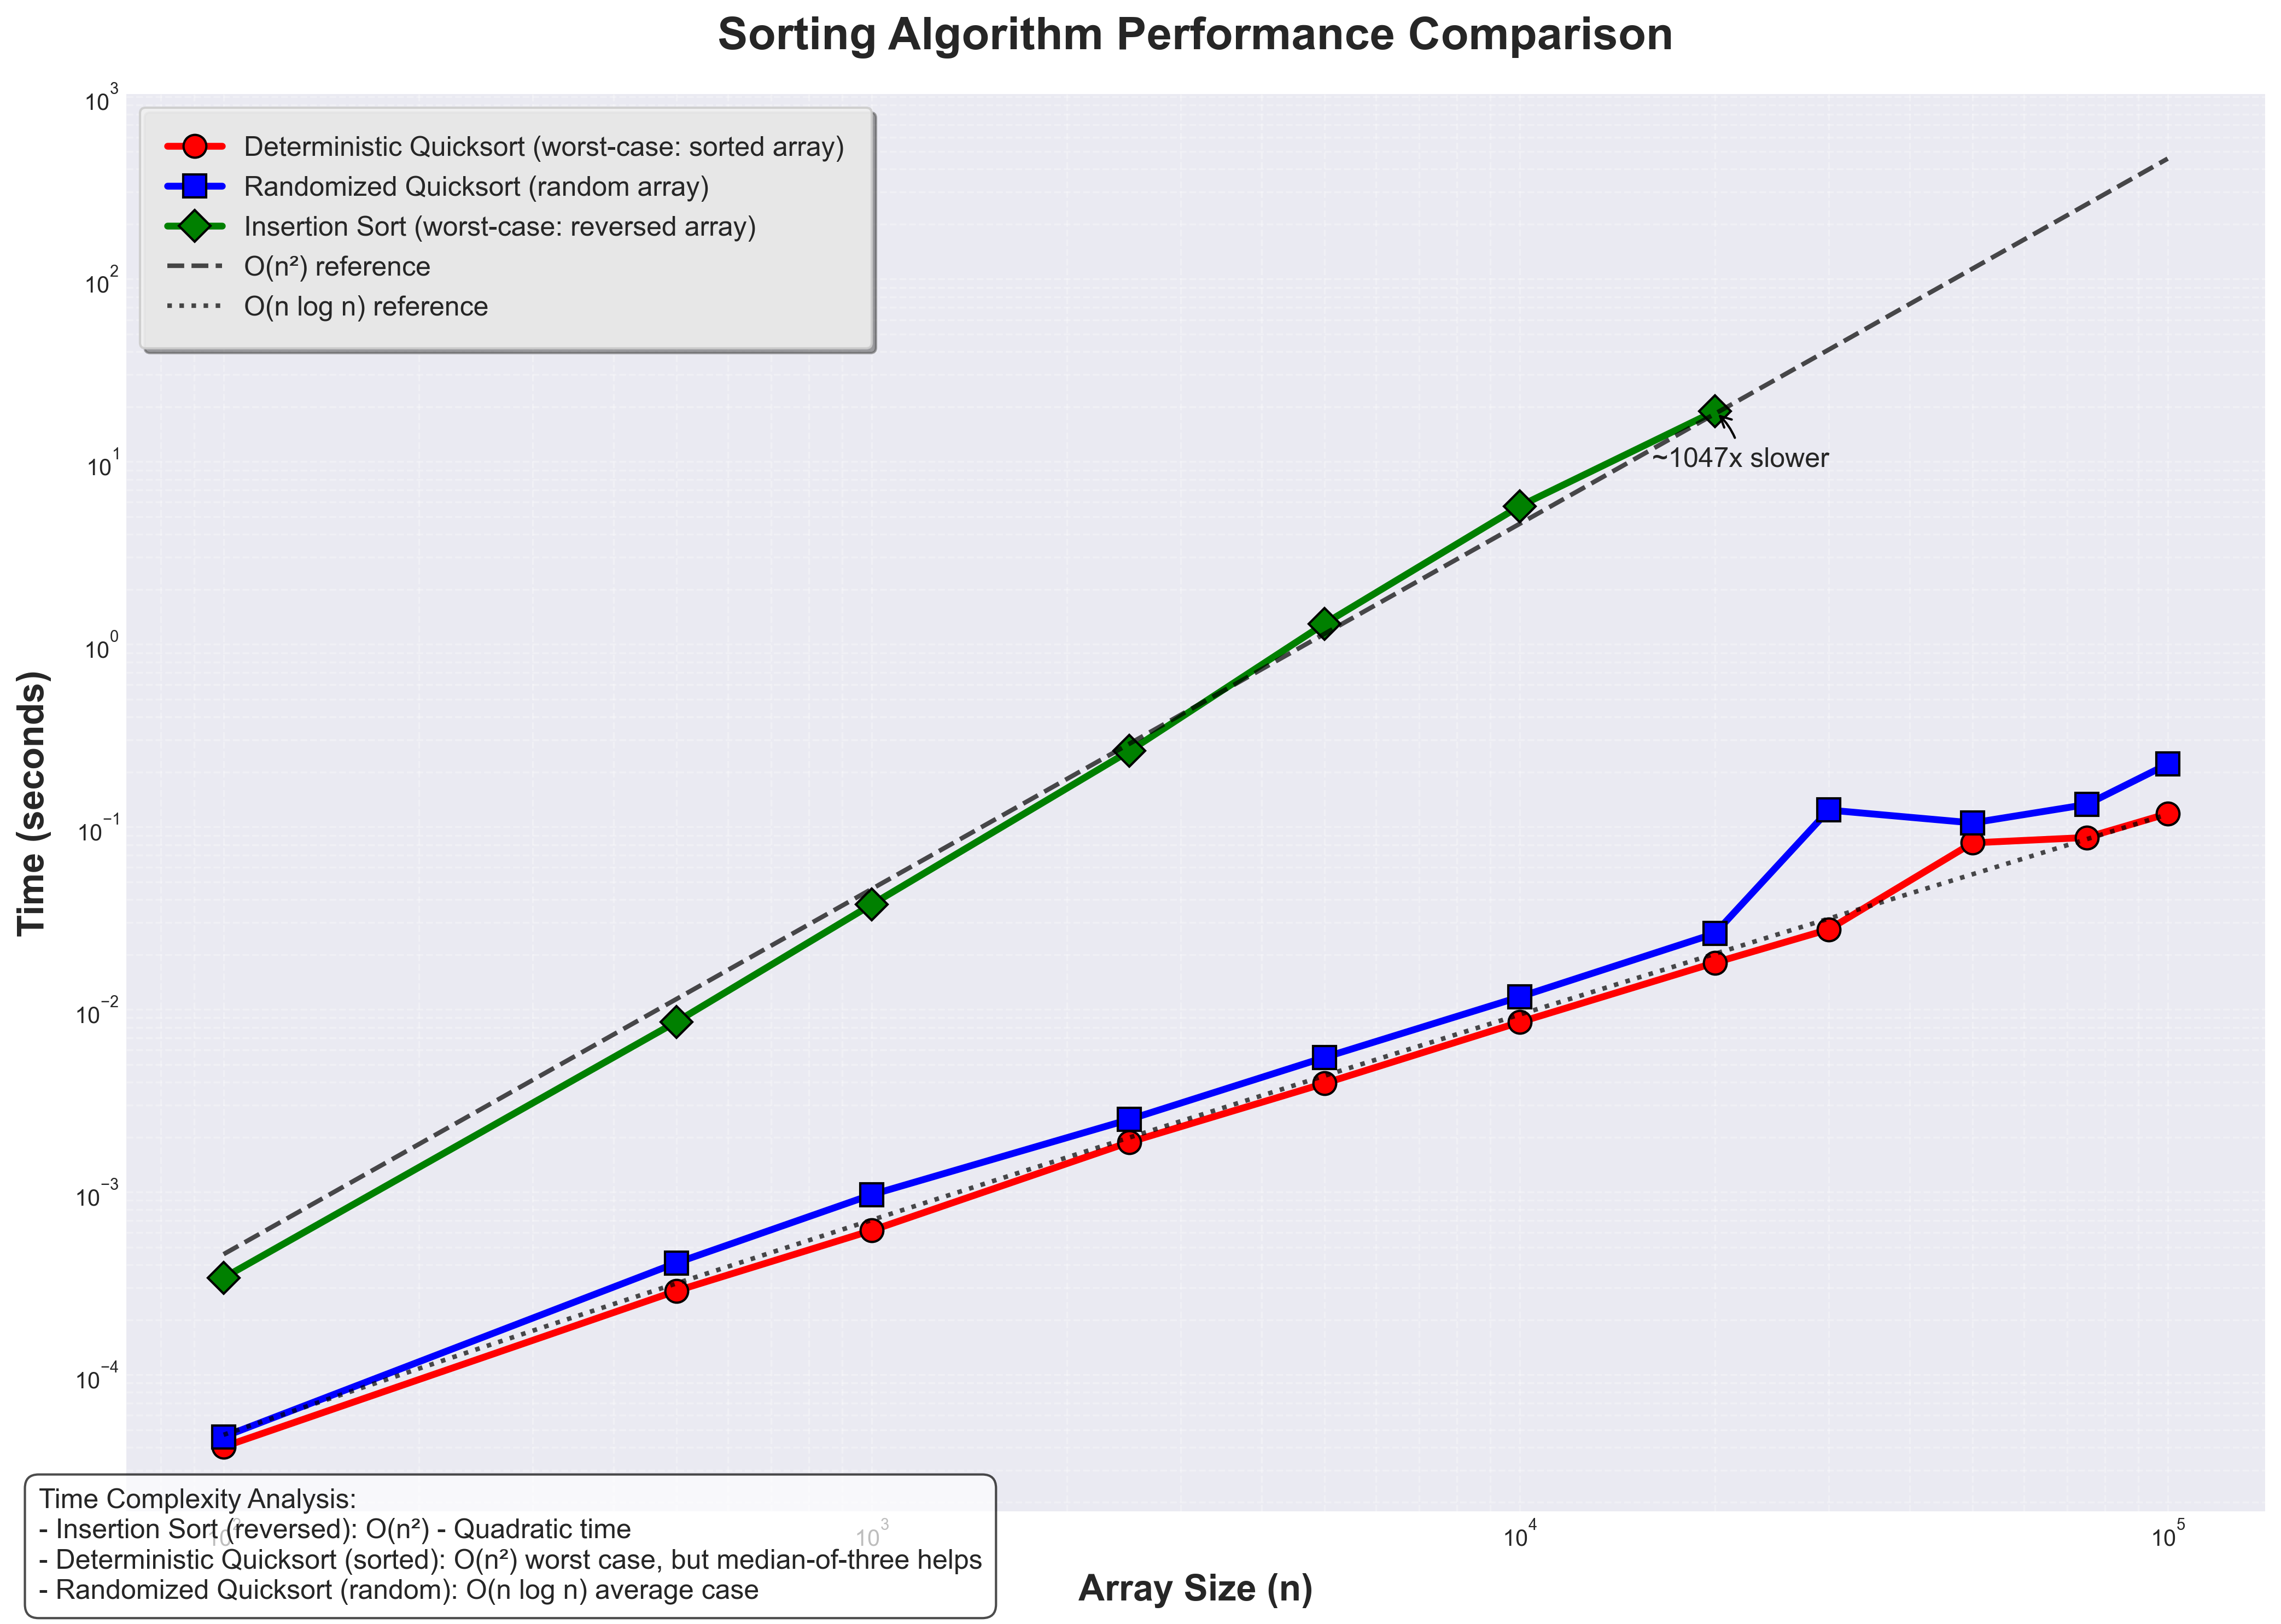
\includegraphics[height=0.95\textheight]{./programs/analysis_quicksort/sorting_algorithms_benchmark.png}
  \end{figure}
\end{frame}

\begin{frame}{Quicksort Recurrence}
  \begin{block}{Expected Comparisons}
    Let $T(n)$ be the expected number of comparisons to sort $n$ distinct elements using randomized quicksort:
    \[
      T(n) \leq n + \frac{1}{n} \sum_{i=1}^n (T(i-1) + T(n-i))
    \]
  \end{block}

  \begin{itemize}
    \item $n$ comparisons in partitioning: each element compared to the pivot.
    \item Pivot is chosen uniformly at random.
    \item For pivot at position $i$, recursive calls sort subarrays of size $i - 1$ and $n - i$.
    \item We average over all $n$ possible pivot positions.
  \end{itemize}

  \begin{block}{Base Case}
    \[
      T(1) = 0 \quad \text{(single element requires no comparisons)}
    \]
  \end{block}

  \begin{block}{Asymptotic Solution}
    Solving the recurrence gives:
    \[
      T(n) = O(n \log n)
    \]
    \parencite{journals/acta/Sedgewick77}
  \end{block}
\end{frame}


\begin{frame}{Solving the Recurrence Step-by-Step}
  \textbf{Step 1: Write the Recurrence}
  \[
    T(n) \leq n + \frac{1}{n} \sum_{i=1}^n (T(i-1) + T(n-i))
  \]
  \textbf{Step 2: Guess the Solution}
  Assume $T(n) \leq cn \log n$ for some constant $c$.

\end{frame}
\begin{frame}{Solving the Recurrence Step-by-Step}
  \textbf{Step 3: Plug the Guess}
  \[
    T(n) \leq n + \frac{2c}{n} \sum_{k=1}^{n-1} k \log k
  \]

  Use:
  \[
    \sum_{k=1}^{n-1} k \log k \leq \frac{1}{2}n^2 \log n - \frac{1}{8}n^2
  \]

  Then:
  \[
    T(n) \leq n + c n \log n
  \]

  \textbf{Step 4: Conclusion}
  \[
    T(n) = O(n \log n)
  \]
\end{frame}